\documentclass[a4paper, 14pt]{article}
\usepackage{fontspec, extsizes, geometry, setspace, titlesec, fancyhdr, graphicx, float, setspace, caption, csquotes, color, listings}
\usepackage[russian, english, ukrainian]{babel}
\usepackage[dotinlabels]{titletoc}
\bibliographystyle{gost-numeric}
\usepackage[backend=biber, bibstyle=gost-numeric]{biblatex}
\addbibresource{paper.bib}
\setmainfont[Ligatures=TeX]{Times New Roman}
\geometry{a4paper,total={170mm,257mm},left=2cm,top=2cm,bottom=2cm,right=2cm}
\def\changemargin#1#2{\list{}{\rightmargin#2\leftmargin#1}\item[]}\let\endchangemargin=\endlist % удобная команда
\makeatletter\newcommand\Dotfill{\leavevmode\leaders\hb@xt@0.65em{\hss.\hss}\hfill}\makeatother % удобная команда
\let\stdsection\section\renewcommand\section{\newpage\stdsection} % Новая секция -> новая страница
\addto\captionsenglish{\renewcommand{\figurename}{Рис.}} % Подпись картинок
\titleformat{\section}[display]{\filcenter}{\bfseries{РОЗДІЛ \thesection.}}{0pt}{\bfseries\MakeUppercase} % Изменение заголовка всех разделов
\renewcommand{\thesubsection}{\arabic{section}.\arabic{subsection}} % Чиним номер подраздела
\titleformat{\subsection}{\filcenter}{\bfseries \thesubsection. }{0pt}{\bfseries}{} %чиним название подраздела 
\captionsetup{labelsep=period} % "Рис. 1." вместо "Рис. 1:"
\fancyhf{}\renewcommand{\headrulewidth}{0pt}\newcommand{\changefont}{\fontsize{14}{14}\selectfont}\fancyhead[R]{\changefont \thepage}\fancypagestyle{plain}{\fancyhf{}\fancyhead[R]{\changefont \thepage}\renewcommand{\headrulewidth}{0pt}\renewcommand{\footrulewidth}{0pt}}\pagestyle{fancy} %номер страницы справа сверху на всех страничках [это ужас]
\linespread{1.25} %#1
\renewcommand{\contentsname}{ЗМІСТ} %изменяем название странички с содержанием
\def\numberline#1{#1. } % Фикс чтобы названия не налезали друг на друга в содержании
\titlecontents{section}[0pt]{\normalfont}{РОЗДІЛ \thecontentslabel. }{}{\Dotfill \contentspage} % точки в содержании
\titlecontents{subsection}[0pt]{\normalfont}{\thecontentslabel. }{}{\Dotfill \contentspage} % точки в содержании
\titlecontents{subsubsection}[2.25em]{\normalfont}{\thecontentslabel. }{}{\Dotfill \contentspage} % точки в содержании
\newcommand{\RNum}[1]{\uppercase\expandafter{\romannumeral #1\relax}}
\definecolor{dkgreen}{rgb}{0,0.6,0}
\definecolor{gray}{rgb}{0.5,0.5,0.5}
\definecolor{mauve}{rgb}{0.58,0,0.82}
\graphicspath{{./images/}}
\lstset{frame=tb, language=Java,  aboveskip=3mm,  belowskip=3mm,  showstringspaces=false,  columns=flexible,  basicstyle={\small\ttfamily},  numbers=none,  numberstyle=\tiny\color{gray},  keywordstyle=\color{blue},  commentstyle=\color{dkgreen},  stringstyle=\color{mauve},  breaklines=true,  breakatwhitespace=true, tabsize=2
}
\lstset{moredelim=[is][\textit]{[*}{*]}}
\begin{document}
% Титулка
\thispagestyle{empty}
\begin{spacing}{1}
\begin{center}
Міністерство освіти і науки України\\
Департамент науки і освіти Харківської облдержадміністрації\\
Харківське територіальне відділення МАН України\\
\end{center}\par\null\par
\begin{changemargin}{10cm}{0cm}
Відділення: комп'ютерних наук\\
Секція: комп'ютерні системи та мережі
\end{changemargin}\par\null\par
\begin{center}
РОЗРОБКА МЕТОДА ПОШУКУ ТА УСУНЕННЯ ПОВТОРЮВАНИХ ЧАСТИН 
У ПОЧАТКОВОМУ КОДІ ПРОГРАМНОГО ЗАБЕЗПЕЧЕННЯ
\end{center}\par\null\par\null
\begin{changemargin}{10cm}{0cm}
Роботу виконав:\\ 
Човпан Ігор Сергійович,\\
учень 11 класу Харківського\\
Навчально-виховного комплексу\\
№45 «Академічна гімназія»\\
Харківської міської ради\\
Харківської області
\end{changemargin}\par
\begin{changemargin}{10cm}{0cm}
Науковий керівник:\\
Руккас Кирило Маркович,\\
професор кафедри теоретичної та\\
прикладної інформатики\\
механіко-математичного\\
факультету Харківського\\
національного університету\\
ім. В.Н. Каразіна, доктор\\
технічних наук, доцент\\
\vspace*{\fill}\end{changemargin}
\begin{center}
Харків -- 2020
\end{center}\end{spacing}

% Тези
\section*{Т\lowercase{ези}}
...
\newpage
\tableofcontents %генерация содержания
\newpage
\section*{\textbf{ВСТУП}}
\addcontentsline{toc}{section}{ВСТУП} %добавляем страницу ВСТУП в содержание
Ваш ВСТУП
\newpage %ну и дальше Ваш ман
\section{Характеристика існуючих методів знаходження повторюваних частин у коді}
Для того щоб проаналізувати методи знахождення повторюваних частин, треба визначити, що таке повторювана частина. \\
Вважатимемо дублікатом фрагмент, який є ідентичним з іншим фрагментом коду. \\
Тоді повторювана частина коду -- фрагмент, в якого є дублікати. \\
Визначемо основні види повторюваних частин.
\subsection{Основних види повторюваних частин}
Як зазначено у роботах \cite{Gautam16}, \cite{Dang15} та \cite{Thummalapenta10}, виділяється 4 головних типи повторюваних частин. 
\begin{itemize}
\item \RNum{1} тип -- повна копія без модифікацій, окрім пробілів та коментарів;
\begin{figure}[!htb]
\centering
\begin{minipage}[t]{.45\textwidth}
\begin{lstlisting}[frame=none]
double xx = Math.cos(angle);
double yy = Math.sin(angle);
xx*=2;
yy*=2;	
if (xx>PI)
	xx = 2*PI-xx;
if (yy>PI)
	yy = 2*PI-yy;
\end{lstlisting}
\end{minipage}
\begin{minipage}[t]{.45\textwidth}
\begin{lstlisting}[frame=none]
double xx = Math.cos(angle);
// of course using math package!!
double yy = Math.sin(angle);
xx *= 2;
yy *= 2;	
if ( xx > PI)
//That is VERY important statement!
	xx = 2 * PI - xx; 
if (yy > PI)
	yy = 2 * PI - yy;
\end{lstlisting}
\end{minipage}
\caption*{Приклад копії \RNum{1} типу на мові Java}
\end{figure}
\item \RNum{2} тип -- синтаксично однакова копія, змінюються лише назви змінних, назв функцій, тощо;
\begin{figure}[!htb]
\centering
\begin{minipage}[t]{.45\textwidth}
\begin{lstlisting}[frame=none]
void func(double angle) {
	double xx = Math.cos(angle);
	double yy = Math.sin(angle);
	xx*=2;
	yy*=2;	
	if (xx>PI)
		xx = 2*PI-xx;
	if (yy>PI)
		yy = 2*PI-yy;
	write(xx);
}
\end{lstlisting}
\end{minipage}
\begin{minipage}[t]{.45\textwidth}
\begin{lstlisting}[frame=none]
void veryImportantFunc(double ang){
	double aa = Math.cos(ang);
	double bb = Math.sin(ang);
	aa*=2;
	bb*=2;	
	if (xx>PI_CONST)
		aa = 2*PI_CONST-aa;
	if (yy>PI_CONST)
		bb = 2*PI_CONST-bb;
	writeToFile(aa);
}
\end{lstlisting}
\end{minipage}
\caption*{Приклад копії \RNum{2} типу}
\end{figure}
\item \RNum{3} тип -- копія з подальшими змінами; доданими, зміненими або видаленими інструкціями;
\begin{figure}
\centering
\begin{minipage}[t]{.45\textwidth}
\begin{lstlisting}[frame=none]
void func(double angle) {
	double xx = Math.cos(angle);
	double yy = Math.sin(angle);
	double PI = Math.acos(-1);
	xx*=2;
	yy*=2;	
	if (xx>PI)
		xx = 2*PI-xx;
	if (yy>PI)
		yy = 2*PI-yy;
	write(xx);
}
\end{lstlisting}
\end{minipage}
\begin{minipage}[t]{.45\textwidth}
\begin{lstlisting}[frame=none]
void doCalc(double ang){
	double bb = Math.sin(ang);
	double aa = Math.cos(ang);
	print("before"+aa);
	aa*=2;
	if (xx>PI_CONST)
		aa = 2*PI_CONST-aa;
	bb*=2;	
	if (yy>PI_CONST)
		bb = 2*PI_CONST-bb;
	print(aa);
}
\end{lstlisting}
\end{minipage}
\caption*{Приклад копії \RNum{3} типу}
\end{figure}
\item \RNum{4} тип -- частина, що робить ідентичні обчислювання, але синтаксично імплементована інакше.
\begin{figure}
\centering
\begin{minipage}[t]{.45\textwidth}
\begin{lstlisting}[frame=none]
int fibonacci(int n) {
	int sum1=0, sum2=1;
	for (int i=2; i<=n; i++){
		int sum3 = sum3+sum2;
		sum1 = sum2;
		sum2 = sum3;
	}
	return sum2;
}
\end{lstlisting}
\end{minipage}
\begin{minipage}[t]{.45\textwidth}
\begin{lstlisting}[frame=none]
int[] mem = new int[...];
int fib(int n) {
	if (mem[n]!=0)
		return mem[n];
	if (n<2)
		return 1;
	mem[n] = fib(n-1)+fib(n-2);
	return mem[n];
}
\end{lstlisting}
\end{minipage}
\caption*{Приклад копії \RNum{4} типу}
\end{figure}
\end{itemize}
\subsection{Основні методи пошуку повторюваних частин}
Існує багато прийомів, що використовуються для пошуку повторюваних частин у початковому коді програмного забезпечення.

Перелічим основні методи пошуку:
\begin{itemize}
	\item пошук збігу рядків початкового коду; 
	\item використання токенів;
	\item метод порівняння функцій;
	\item застосування графа програмних залежностей;
	\item метод порівняння дерев.
\end{itemize}
Далі визначимо усі переваги і недоліки кожного з методів.

\subsubsection{Пошук збігу рядків початкового коду}
Обчислюється ступінь схожості для кожної пари рядків за допомогою відстані Левенштейна. Емпірично встановлюється мінімальна величина, за якої вважається, що 2 рядки є копіями одна одну. 

Переваги цього метода:  
\begin{itemize}
\item добре знаходить копії \RNum{1} типу;
\item невеликий час виконання порівняно з іншими методами;
\item підтримка будь-якої мови программування.
\end{itemize}

Недоліки метода:
\begin{itemize}
\item велика кількість хибнонегативних результатів;
\item нестійкість до різних "шумів": коментарів, змінених назв функцій або змінних, тобто неможливість знайти дублікати \RNum{2} та \RNum{3} типу. 
\item Не враховуються особливості мови програмування.
\end{itemize}
Прикладом використання є програма PMD.
\subsubsection{Використання токенів}
Початковий код розбивається на токени, при пошуці порівнюються послідовності токенів.
Головною перевагою цього методу є стійкість до переформатування початкового коду, зміні назв змінних.
Недоліком є те, що токенізатори враховують тільки базові особливості мови програмування, тому багато послідовностей, які вважаються копіями, насправді самі по собі не мають сенсу. \cite{Koschke06}
\begin{figure}[h!]
\centering
\begin{minipage}[t]{.275\textwidth}
\begin{lstlisting}[frame=none]
return x;
void func(int y) {
  y++;
\end{lstlisting}
\end{minipage}
\begin{minipage}[t]{.275\textwidth}
\begin{lstlisting}[frame=none]
return a;
void myFunc(int b) {
  b++;
\end{lstlisting}
\end{minipage}
\begin{minipage}[t]{.35\textwidth}
\begin{lstlisting}[frame=none]
void,myFunc,(,int,b,),{,b,++,;
\end{lstlisting}
\end{minipage}
\caption*{Частини коду, що вважатимуться копіями; приклад розбиття коду на токени}
\end{figure}
Прикладом використання такого методу є програма CCFnderX. 
\subsubsection{Метод порівняння функцій}
За допомогою парсера мови програмування знаходять усі функції у початковому коді. Далі усі ці функції порівнюються між собою або за допомогою спеціально обраної "поганої" геш-функції, або за допомогою обчислення коефіцієнту схожості (наприклад, коеф. Жаккара).
Метод гарно знаходить збіги між різними функціями, розпізнаються копії \RNum{1}-\RNum{3} типу, проте він не може знайти повторювани частини всередині коду.
Прикладом використання є \cite{Yang18}.
\subsubsection{Застосування графа програмних залежностей}
Згідно з \cite{Ferrante87}, граф програмних залежностей (далі просто граф) -- представлення програми як графа, у якому кожна вершина - інструкція у програмі, а також зв'язані з цією інструкцією оператори та операнди; ребрами у такому графі є дані, від яких залежить виконання цієї інструкції та умови, за яких ця інструкція виконається.
\begin{figure}[h]
    \centering
    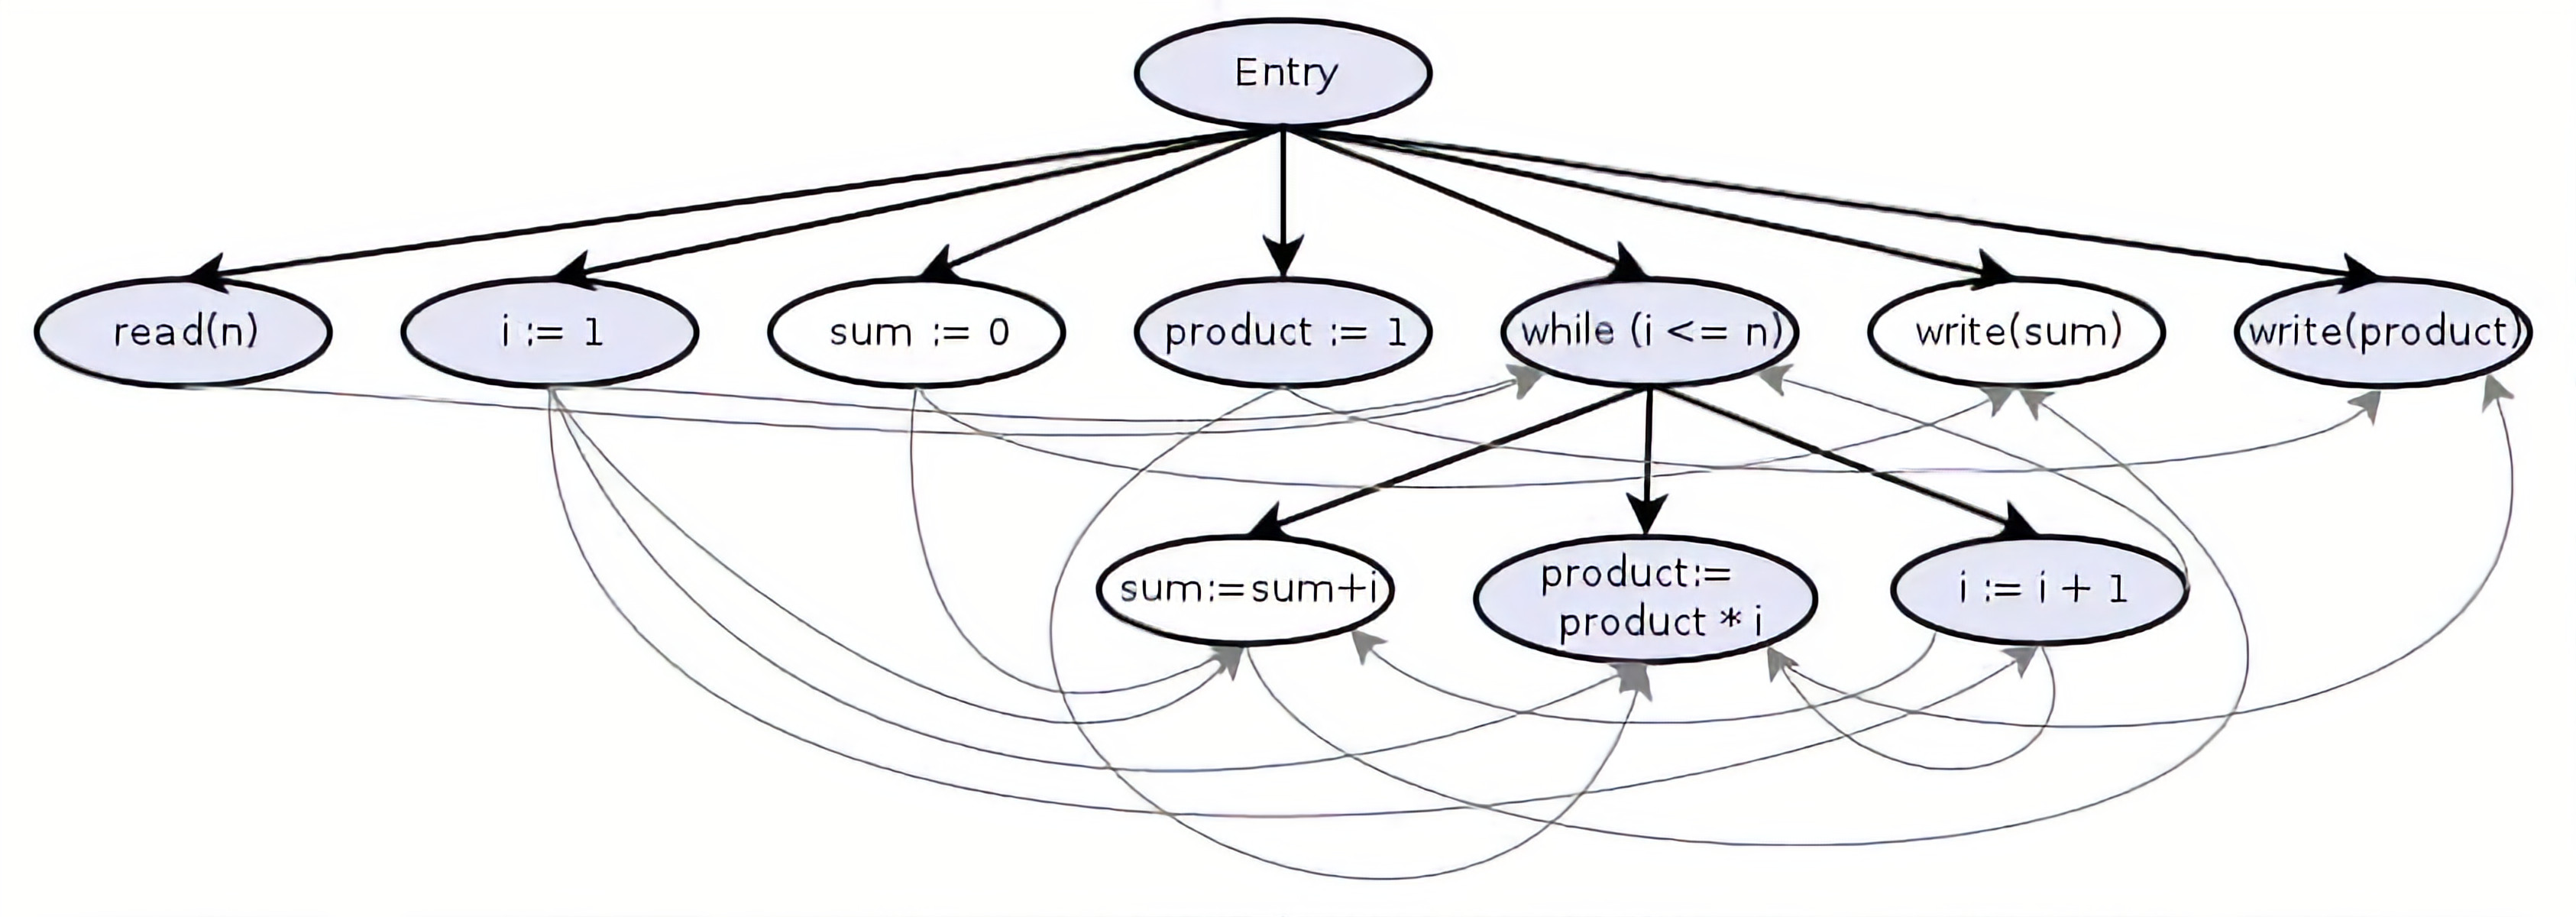
\includegraphics[width=0.75\textwidth]{pdg-example}
    \caption{Приклад графа програмних залежностей \cite{pdg-example}}
    \label{fig:pdg-example}
\end{figure} 
Дві частини програми вважаються ідентичними, якщо їх графи ізоморфні.
Головною перевагою є те, що цей граф не залежить від переставлення інструкції програми; зміни назв функцій, змінних, тощо; не залежить від аспектів реалізації.
Недоліки методу:
\begin{itemize}
\item Дуже довгий час роботи, оскільки завдання пошуку ізоморфних підграфів є NP-повною, і може бути вирішена за поліноміальний час тільки для планарних графів, що не обов'язково виконається для графа програмних залежностей;
\item Такий метод не зможе знайти дублікати у коді, який не виконується у загальному випадку, оскільки у граф додаються лише виконані інструкції.
Приклад використання: \cite{Liu06}.
\end{itemize}
\subsubsection{Метод порівняння дерев}
У цьому методі використовуються абстрактні синтаксичні дерева (АСД). Згідно з \cite{wiki:ast}, абстрактне синтаксичне дерево -- позначене і орієнтоване дерево, в якому внутрішні вершини співставлені з відповідними операторами мови програмування, а листя з відповідними операндами.
\begin{figure}[h!]
    \centering
    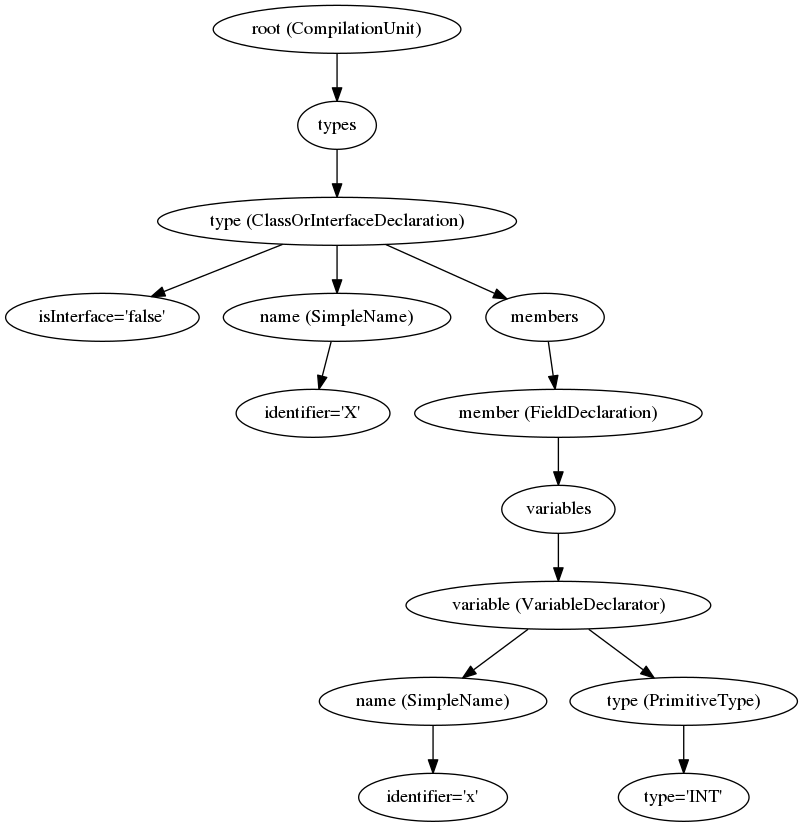
\includegraphics[width=0.75\textwidth]{ast-example}
    \caption{Приклад абстрактного синтаксичного дерева \cite{ast-example}}
    \label{fig:pdg-example}
\end{figure}\\
Щоб визначити, чи є частина коду копією іншої частини, знаходять відповідні їм піддерева, а далі ці піддерева порівнюються між собою. \\
Підходів порівяння піддерев досить багато. Так, наприклад, у роботі \cite{Sager06} усі піддерева, що відповідають класам у початковому коді, порівнюються кожен з кожним за допомогою обчислення відстані між деревами. Автор відмічає, що цей метод є найточнішим порівняно з іншими, але має дуже довгий час роботи. Наприклад, код плагінів \verb|org.eclipse.compare-plug-in|, що складався зі 114 класів перевірявся на копії більше ніж годину. \\
У роботі \cite{Baxter98} теж стверджується, що алгоритм знахождення між деревами має занадто велику складність обчислення, тому автором було запропоновано інший підхід. Усі піддерева гешуються за допомогою вибраної "поганої" геш-функції та розподіляються у $B$ бакетів, де $B \approx N/10$. 
Далі кожне піддерево порівнюється лише з піддеревами з цього ж бакету за формулою: $$\textup{Схожість} = \frac{2*S}{2*S+L+R}.$$ $S$ -- кількість однакових вершин у обох піддеревах, $L$ -- кількість вершин, що присутні лише у першому піддереві, $R$ -- кількість вершин, що є тільки у другому піддереві. \\
Отже, головними перешкодами до використання цього методу є:
\begin{itemize} 
\item Великі час роботи та алгоритмічна складність; \cite{Ain19}
\item Досить низький відсоток знайдених копій через використання додаткових евристик. \cite{Dang15}
\end{itemize}
Далі буде запропоновано новий підхід, що значно зменшить час роботи, необхідний для знаходження копій, та, у той же час, збільшить ефективність їх знаходження.
\section{Новий алгоритм}
Алгоритм складається із 4 кроків:
\begin{enumerate}
\item парсинг коду та перетворення його у абстрактне синтаксичне дерево;
\item визначення частин коду, які має сенс порівнювати;
\item знаходження повторюваних частин;
\item перетворення знайденого результату до конкретних елементів у коді.
\end{enumerate}
Далі опишемо детальніше кожен крок.
\subsection{Парсинг коду}
Компілятор практично будь-якої мови програмування на якомусь кроку перетворює код у абстрактне синтаксичне дерево. Для простоти, будемо працювати з кодом, написаним на мові програмування Java. Щоб перетворити код у абстрактне синтаксичне дерево, використаємо JavaParser. Алгоритм не складно змінити для підтримки будь-якої іншої мови програмування.
\subsection{Визначення частин коду, які підлягають порівнянню}
У загальному випадку, структура коду у об'єктно-оріентованих мовах программування виглядає таким чином: \\
\begin{lstlisting}[frame=none, xleftmargin=.3\textwidth]
import com.google.tools;
class X {
	int a=0;
	X(int a, int b)	{
		this.a = a;
	}
	void incrementAndPrint()	{
		a++;
		print(a);
	}
}
\end{lstlisting}
Із прикладу можна визначити головні елементи практично кожної програми, а саме:
\begin{itemize}
\item підключення інших пакетів, бібліотек;
\item декларування класу та його елементи (поля);
\item декларування функцій та обчислення якогось результату.
\end{itemize}
Будемо вважати, що порівнянню і подальшому опрацюванню підлягають лише ті частини коду, які можна винести до іншої функції.
Цими елементами є тільки ствердження у функціях.\\
Пояснемо на прикладі: \\
\begin{figure}[h!]
\begin{lstlisting}[frame=none, xleftmargin=.3\textwidth]
import com.google.tools;
class X {
	int a=0;
	X(int a)	{
		[*this.a = a;*]
	}
	void incrementAndPrint()	{
		[*a++;
		print(a);*]
	}
}
\end{lstlisting}
\caption*{Приклад коду}
\end{figure} \\
Курсивом виділені фрагменти коду, що будуть далі опрацьовані. \\
Визначимо вираз як найменша неподільна операція та параметр до цієї операції. \\ Будь яке велике обчислення можна розбити на вирази. \\
У операціях розгалуження вважатимемо виразами лише додаткові умови у них, але не самі операції. \\
Блок -- непорожня послідовність виразів, укладених між фігурними дужками та впорядкованих за порядком обходу алгоритма DFS у абстрактному синтаксичному дереві. \\
Алгоритм розбиває код на блоки таким чином, що вміст одного блоку не зустрічається у іншому. \\
\begin{figure}[h!]
\centering
\begin{minipage}{.4\textwidth}
\begin{lstlisting}[frame=none]
void func(){
	int x = 10;
	x = x+1;
	while (x>3){
		System.out.println(x*2);
		x--;
	}
}
\end{lstlisting}
\end{minipage}
\begin{minipage}{.5\textwidth}
\begin{lstlisting}[frame=none]
[int x = 10;, x = x + 1;, x > 3, System.out.println(x * 2);, x--;]
\end{lstlisting}
\end{minipage}
\caption*{Приклад розбиття коду на вирази у блоці}
\end{figure} \\ \null \\
Порівнянню з іншою послідовністю підлягає будь-яка послідовність виразів, що йдуть поспіль, та знаходяться у одному блоці. \\
\subsection{Знаходження повторюваних частин}
\subsection{Перетворення до елементів у коді}
\section{Порівняння з іншими методами}
...
\section{Висновки}
...
\printbibliography[title={список використаних джерел}]
\end{document}
